\documentclass[]{IEEEtran}

\title{Software fast parallel calculation of 32-bit Cyclic Redundancy Check using Cuda}
\author{Francesco Tosoni, Nereo Sorio}

\usepackage{graphicx}
\usepackage[english]{babel}

\begin{document}
\maketitle

\begin{abstract}
Questo documento serve come traccia per la relazione da consegnare come primo assignment del corso di Progettazione di Sistemi Embedded. Si ricorda che la relazione va consegnata insieme al codice sorgente delle soluzioni.

Il sommario, o abstract, conterr\`a una brevissima descrizione degli obiettivi del progetto, delle caratteristiche principali del flusso di progettazione e dei risultati principali ottenuti. 
\end{abstract}


\section{Introduction}

CRC (\emph{Cyclic Redundancy Check}) is a checksum algorithm to detect inconsistency of data, e.g. bit errors during data transmission. Blocks of data can therefore be checked quickly, based on the remainder of a polynomial division. The calculation is then performed both by the transmitter, which appends its result to the data, and by the receiver, which compares its result with the transmitted one. This technique is very effective in detecting physical errors on the transmission channel, but not in against intentional corruption of data. 

The encoding of a CRC value requires a \textbf{generator polynomial} to be defined. It will serve as a \textbf{divisor} in a \textbf{long division}, in which the data to be transmitted becomes the dividend. In this case, the quotient is of no use and therefore is discarded, while the \textbf{remainder is the CRC value}. 
The polynomial coefficients are calculated according to the arithmetic of a finite field, so there is no carry between digits. Obviously, as shown in the next section, the message is also encoded as a polynomial. 

When talking about $n$-bit CRC, $n$ is the size of the checksum value. There are several protocols for a CRC of size $n$ but with different values: simply, the generator polynomial changes. 
Traditional algorithms are implemented through cyclic operations, since many times, the CRC is calculated at hardware level. The checksum value in fact, is obtained with a few simple operations repeated on each block (of fixed size) of data. 
The simplest error-detection system, the parity bit, is in fact a 1-bit CRC: it uses the generator polynomial x + 1 (two terms).

\section{Background}

The CRC value is usually calculated on a fixed-length
bit stream. 

\section{Serial Algorithms}

In questa sezione viene descritto tutto il procedimento, ed \`e dunque la sezione pi\`u importante del report. Va descritto passo passo quello che avete fatto, facendo capire ``esattamente'' cosa \`e stato fatto.

Questa sezione pu\`o essere divisa in sottosezioni. Le informazioni riportate nella lista seguente dovrebbero essere identificabili nel testo del report (\textbf{anche in ordine diverso}):
\begin{itemize}
\item Definizione dell-architettura del programma
\item Descrizione del componente di HW digitale.
\item Processo di ``sintesi'' verso RTL. Definizione dei sottocomponenti del componente HW, e della sua struttura. Definizione dell'interfaccia RTL, definizione della Macchina a Stati Finiti Estesa (EFSM) del componente e dei sottocomponenti. Realizzazione del componente HW utilizzando i processi in diversi stili a livello RTL. \`E inoltre possibile discutere la scelta dei tipi di dato.
%\item Descrizione della realizzazione della parte rappresentante SW Embedded, e descritta in TLM.
%\item Descrizione della realizzazione della parte a tempo continuo. Spiegazione delle scelte progettuali fatte per gli stili di modellazione utilizzati.
\item Descrizione dei meccanismi di comunicazione tra le diverse parti del sistema.
\end{itemize}

\textbf{In questa sezione deve essere riportato (brevemente) anche l'organizzazione dell'implementazione consegnata assieme al report.}

\section{Parallel Algorithms}

\section{Results}

Qua vanno ``messi i numeri''. Questa sezione dovrebbe contenere i risultati della simulazione. La simulazione mostra che il sistema funziona correttamente? Come \`e stato provato? Che tipo di testbench sono stati utilizzati? Come \`e stato scomposto il sistema per verificarne la correttezza?

Per quanto riguarda le performance:
\begin{itemize}
\item cosa si pu\`o dire in merito alla latenza?
\item Qual è la frequenza massima del design? 
\item Qual è l'area occupata dal design? 
\end{itemize}

Questa sezione pu\`o contenere anche riflessioni personali sui risultati ottenuti. Importante: tutte le affermazioni devono essere supportate da numeri\footnote{Richard Feynman on Scientific Method (1964) -\\ https://www.youtube.com/watch?v=OL6-x0modwY}.

\section{Conclusions}
Le conclusioni dovrebbero riassumere in poche righe  tutto ci\`o che \`e stato fatto. Un paio di righe descrivono i risultati osservati, in modo da introdurre poi la conclusione ``vera e propria''. Nel caso del corso, la ``lezione da portare a casa'' sar\`a quello che si \`e imparato svolgendo l'elaborato.


\bibliographystyle{IEEEtran}
\bibliography{biblio}

\appendix
Se non avete abbastanza spazio, potete inserire le figure delle EFSM in una  pagina extra, appendice. Un esempio di come potete fare solo le Figure~\ref{fig:grande}, \ref{fig:piccola1}, \ref{fig:piccola2}.


\begin{figure*}[bt]
\centering
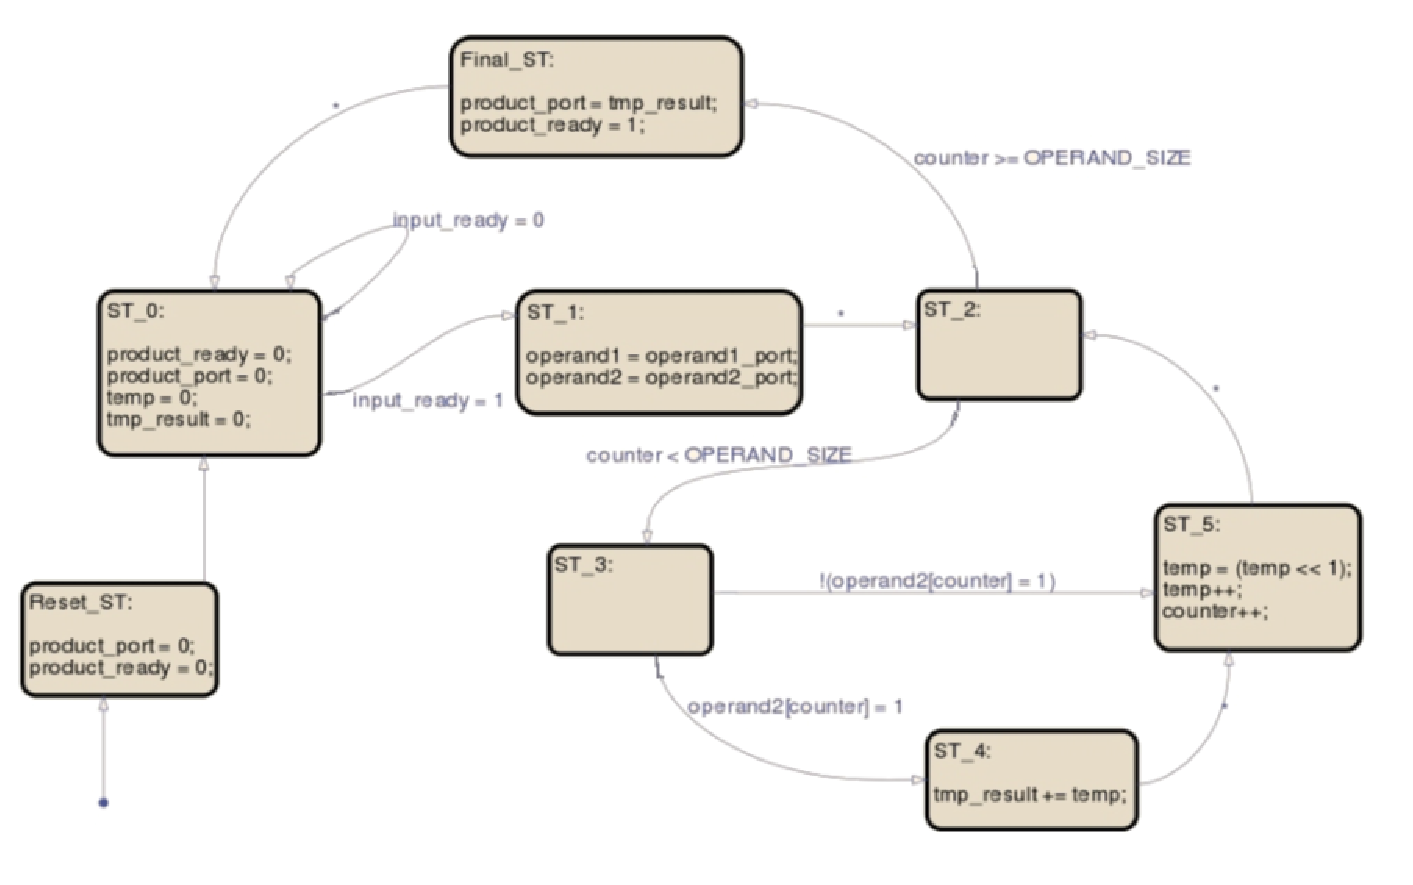
\includegraphics[width=\textwidth]{figures/EFSM}
\caption{Figura in formato grande.}
\label{fig:grande}
\end{figure*}

\begin{figure}[bt]
	\centering
	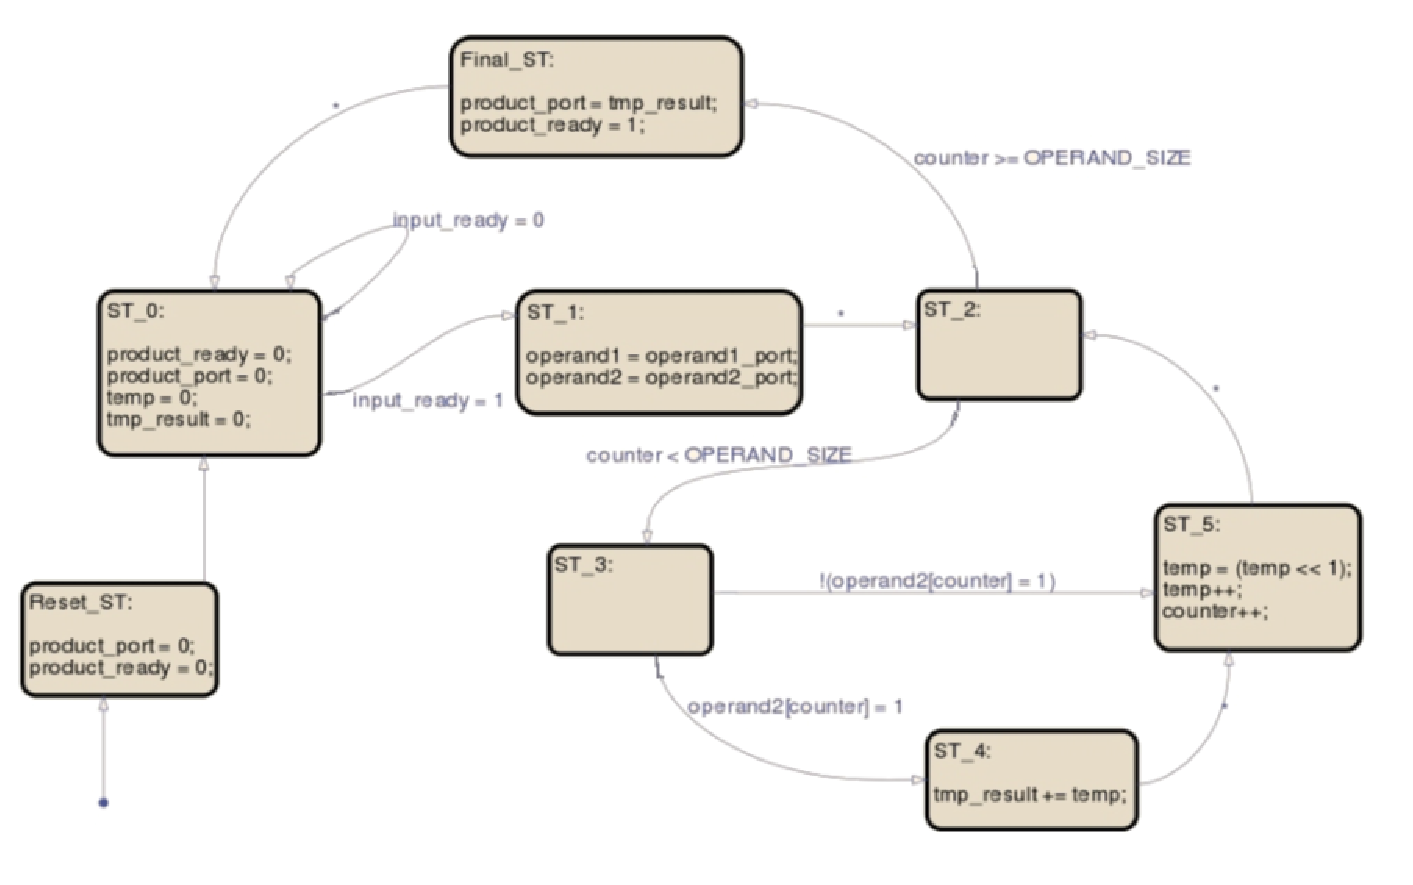
\includegraphics[width=\columnwidth]{figures/EFSM}
	\caption{Figura in formato piccolo, 1.}
	\label{fig:piccola1}
\end{figure}

\begin{figure}[bt]
	\centering
	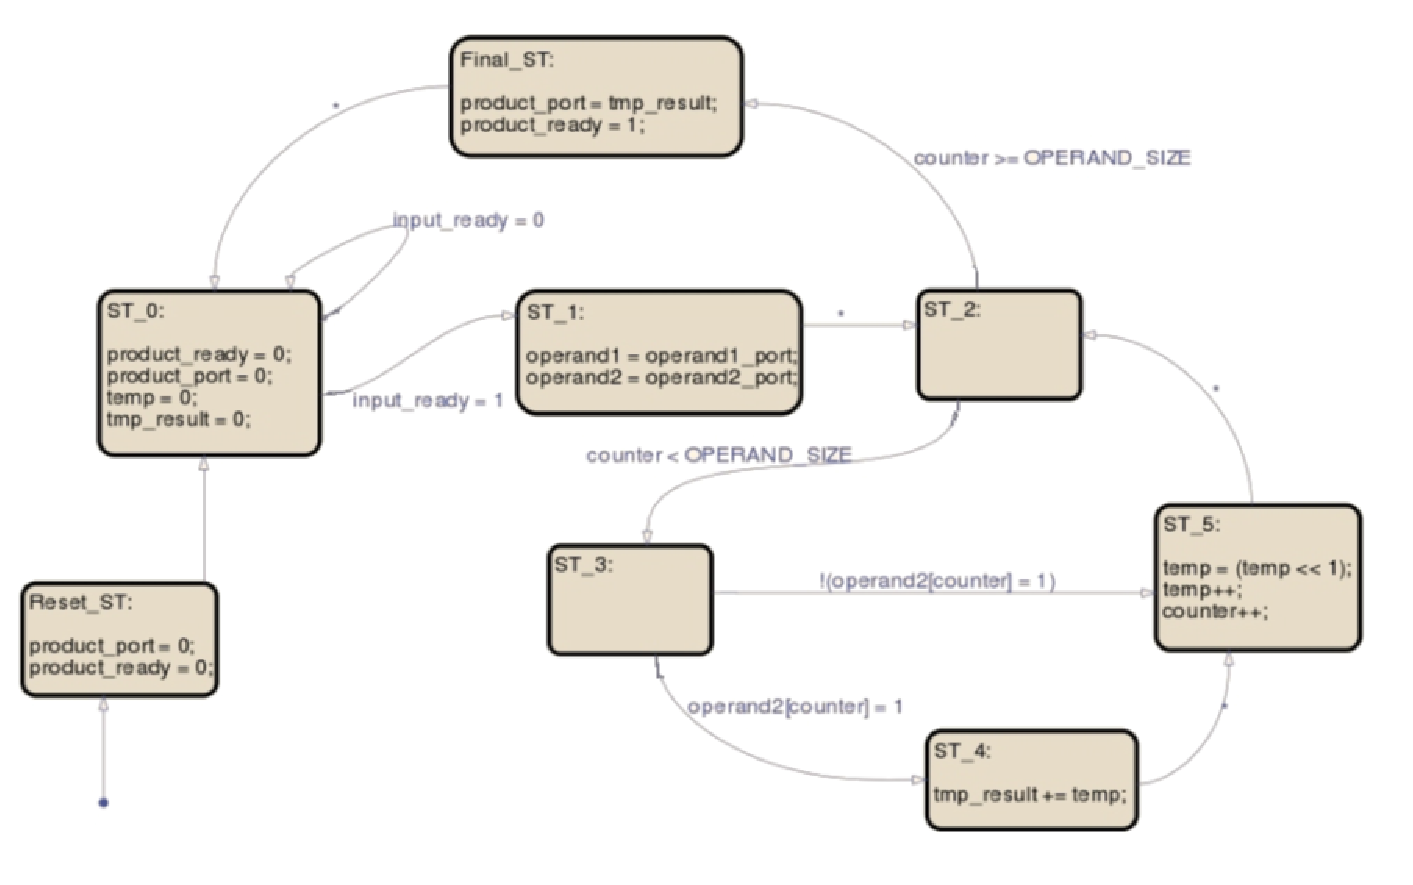
\includegraphics[width=\columnwidth]{figures/EFSM}
	\caption{Figura in formato piccolo, 2.}
	\label{fig:piccola2}
\end{figure}

\end{document}